\chapter{The quasi-local approach: trapping horizons}
\label{s:loc}

\minitoc

\section{Introduction}

This chapter is in a draft stage.

\section{Trapped surfaces and singularity theorems}

\subsection{Trapped surfaces}

The concept of trapped surfaces has been introduced in Sec.~\ref{s:neh:trapped_surfaces}
(see in particular Fig.~\ref{f:neh:trapped_surf}). Let us recall that
a submanifold $\Sp$ of a $n$-dimensional spacetime ($n\ge 3$) is
a \defin{trapped surface}\index{trapped!surface} iff (i) $\Sp$ is a compact $(n-2)$-dimensional manifold
(without boundary), (ii) $\Sp$ is spacelike (positive definite induced metric)
and the two systems of null geodesics emerging orthogonally from $\Sp$ towards the future
locally converge, i.e. they have negative expansions at $\Sp$:
$\theta_{(\wl)} < 0$ and $\theta_{(\w{k})} < 0$ [Eq.~(\ref{e:neh:def_trapped_surf})],
$\wl$ and $\w{k}$ being
future-directed vectors tangent to these geodesics.

\begin{remark}
Trapped surfaces are sometimes called
\emph{closed trapped surfaces}\index{closed!trapped surface}\index{trapped!surface!closed --} (e.g. \cite{Penro65,HawkiE73}),
to stress their closed manifold aspect (compact without boundary).
We follow here the textbooks \cite{MisneTW73,Wald84} and call them merely
\emph{trapped surfaces}.
\end{remark}

\begin{example}[trapped surfaces in Schwarzschild spacetime]
Let $(\M,\w{g})$ be the Schwarzschild spacetime as defined in Sec.~\ref{s:sch:time_orientation} [Eq.~(\ref{s:sch:def_Schwarz_spacetime})]; it is entirely covered by the ingoing Eddington-Finkelstein coordinates
$(\ti,r,\th,\ph)$. Let $\Sp$ be any surface $(\ti,r) = \mathrm{const}$.
$\Sp$ is diffeomorphic to $\mathbb{S}^2$ and thus compact.
Moreover, from Eq.~(\ref{e:sch:Schwarz_metric_EF}), the metric induced by $\w{g}$
on $\Sp$ is $\w{q} = r^2 (\D\th^2 + \sin^2\th\D\ph^2)$, which is clearly positive definite, so
that $\Sp$ is spacelike. One reads also on the expression of $\w{q}$
that the area of  $\Sp$ is simply $A = 4\pi r^2$ (i.e. $r$ is the areal radius, cf. Sec.~\ref{s:sch:static_spher}).
If $\Sp$ is located in the black hole interior, i.e. if $0<r < 2m$,
Property~\ref{p:sch:r_decreasing} implies that $A$ is decreasing along any future-directed null
geodesic. It follows that $\Sp$ is trapped. On the contrary, if located in the black hole exterior
($r> 2m$), $\Sp$ is untrapped. This can be checked on Fig.~\ref{f:sch:rad_null_geod_EF},
where it appears clearly that, in the region $r>2m$, $r$ is increasing along the outgoing radial null geodesics, which are normal to $\Sp$.
\end{example}

\begin{figure}
\centerline{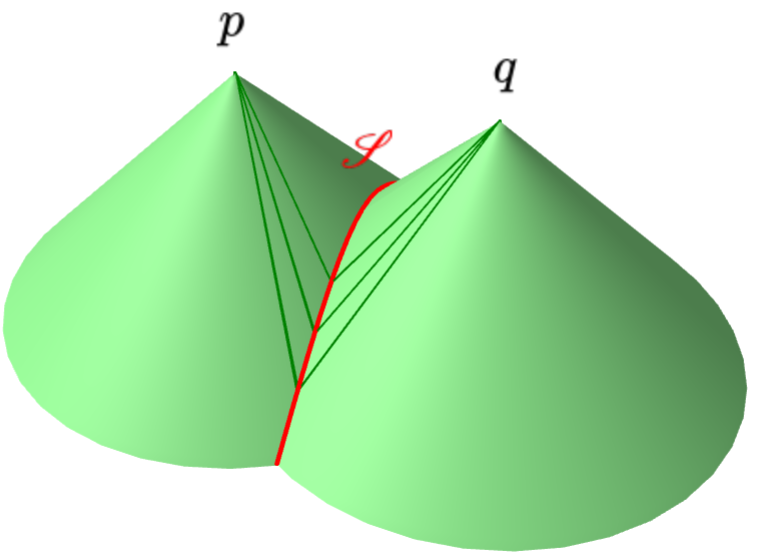
\includegraphics[width=0.6\textwidth]{loc_cone_intersect.png}}
\caption[]{\label{f:loc:cone_intersect} \footnotesize
Intersection $\Sp$ (red curve) of the past light cones of two points $p$ and $q$ in Minkowski spacetime.
Some light rays emerging from $\Sp$ in the two orthogonal null directions are depicted; the two sets
of light rays are both converging. Yet $\Sp$ is not trapped because it is not compact.
\textsl{[Figure generated by the notebook \ref{s:sam:loc_cone_intersect}]}
}
\end{figure}

The existence of a trapped surface is a characterization of
strong gravity\index{gravity!strong --}. More precisely it indicates that gravity is strong enough
to focus all light rays emitted from the surface.
This characterization is \emph{quasi-local}\index{quasi-local}, in the sense that it involves a \emph{surface}. The
surface can be ``small'' but it cannot be reduced to a point, to which the qualifier \emph{local}
would apply. Note that the hypothesis of \emph{compact} manifold is crucial in the definition of a
trapped surface. Without it, trapped surfaces would exist in Minkowski
spacetime, as the following example shows.

\begin{example}[a counter-example in Minkowkski spacetime]
Let us consider the intersection $\Sp$ of the past light cones $\mathscr{C}_p$ and $\mathscr{C}_q$
of two points $p$ and $q$ of Minkowski spacetime (cf. Fig.~\ref{f:loc:cone_intersect}).
Being a cross-section of the null hypersurface $\mathscr{C}_p$ (or $\mathscr{C}_q$),
$\Sp$ is a spacelike surface (Property~\ref{p:def:spacelike_cs}).
Moreover the null directions $\w{k}$ and $\wl$ normal to it are given by the null generators of
$\mathscr{C}_p$ (since $\Sp$ is a cross-section of $\mathscr{C}_p$)
and of $\mathscr{C}_q$ (since $\Sp$ is a cross-section of $\mathscr{C}_q$).
Because $\mathscr{C}_p$ and $\mathscr{C}_q$ are past light cones, one has clearly
$\theta_{(\wl)} < 0$ and $\theta_{(\w{k})} < 0$.
However, $\Sp$ fails to be a trapped surface for it is not compact. Truncating the light cones
would not help, because this would make $\Sp$ a manifold with boundary and hence not a closed one.
\end{example}


\subsection{Penrose's singularity theorem}

Trapped surfaces are the key ingredient of Penrose's singularity theorem,
which basically states that, modulo some assumptions, if gravity is
strong enough that a trapped surface occurs, then some singularity will
appear in the future of it.
Before stating the theorem, let us recall a few concept on which it relies.

First of all, a \defin{Cauchy surface}\index{Cauchy!surface}
$\Sigma$ of a spacetime $(\M,\w{g})$ is a spacelike
hypersurface such that every inextendible timelike curve of $\M$
intersects $\Sigma$ exactly once (cf. Sec.~\ref{s:sta:BH_stationary}). If $(\M,\w{g})$
admits a Cauchy surface, it is said to be a
\defin{globally hyperbolic}\index{globally!hyperbolic} spacetime.
On such a spacetime, general relativity can be formulated as a well posed
Cauchy problem \cite{ChoquG69},
i.e. there exists a unique solution $\w{g}$ of the Einstein equation
in $\M$ from initial data prescribed on $\Sigma$, provided that the initial data
fulfill four components of the Einstein equations known as the
\emph{constraint equations}\index{constraint!equations}.

The second concept involved in Penrose's theorem is that of
an \emph{inextendible incomplete} geodesic. As stated in
Appendix~\ref{s:geo} (Sec.~\ref{s:geo:existence_uniqueness}), a
geodesic $\Li$ of a spacetime $(\M,\w{g})$ is \defin{incomplete}\index{incomplete geodesic}\index{geodesic!incomplete --} if some affine parameter $\lambda$ does take all
possible real values along the whole of $\Li$.
Given that any two affine parameters are related by
an affine transformation, if this holds for a given affine parameter, this holds for all.
More precisely, if $\Li$ is a causal (i.e. timelike or null) geodesic and $\lambda$ is increasing to the future, one says that $\Li$
is \defin{future-incomplete}\index{future!incomplete geodesic}\index{geodesic!future-incomplete --}\index{incomplete!future -- geodesic} if, and only if, $\lambda$ spans the interval
$(-\infty,\lambda_{\rm max})$ along $\Li$, for some $\lambda_{\rm max}\in\R$.
Similarly, one says that $\Li$
is \defin{past-incomplete}\index{past!incomplete geodesic}\index{geodesic!past-incomplete --}\index{incomplete!past -- geodesic} if, and only if,
$\lambda\in(\lambda_{\rm min},+\infty)$ along $\Li$, for some $\lambda_{\rm min}\in\R$.
Furthermore, a geodesic $\Li$ is said \defin{inextendible}\index{inextendible geodesic}\index{geodesic!inextendible --} if, and only if,
there does not exist any geodesic $\Li'$ of $(\M,\w{g})$ distinct from $\Li$
and such that $\Li\subset\Li'$. An inextendible incomplete causal geodesics
marks the existence of a singularity\index{singularity} of some kind. For instance the existence of an
inextendible future-incomplete timelike geodesic $\Li$ implies that the free-falling
observer having $\Li$ as worldline has his proper time\footnote{Recall that
the proper time is an affine parameter along a timelike geodesic (Property~\ref{p:geo:proper_time_affine}).} to abruptly
stop at a some finite value!
We shall discuss this further on later; for the moment, we have enough material
to state the singularity theorem:

\begin{prop}[Penrose's singularity theorem \textnormal{(Penrose 1965 \cite{Penro65})}]
Let $(\M,\w{g})$ be a $n$-dimensional spacetime ($n\ge 3$) such that
\begin{itemize}
\item $(\M,\w{g})$ admits a non-compact Cauchy surface $\Sigma$;
\item the null energy condition (\ref{e:neh:null_energy_cond}) holds on $\M$:
for any null vector $\wl$, $\w{R}(\wl, \wl) \geq 0$, where $\w{R}$ is
$\w{g}$'s Ricci tensor;
\item there exists a trapped surface $\Sp$.
\end{itemize}
Then there exists at least one null geodesic emerging orthogonally from $\Sp$
that is inextendible and future-incomplete.
\end{prop}

\begin{proof}
We shall prove the theorem by contradiction. Hence let us assume that all
null geodesics emerging orthogonally from $\Sp$ are future-complete. Let $\mathscr{F}$
be the boundary of the causal future of $\Sp$
(cf. Sec.~\ref{s:glo:causal_struct}): $\mathscr{F} = \partial J^+(\Sp)$.
$\mathscr{F}$ is a so-called \defin{achronal boundary}\index{achronal!boundary}\index{boundary!achronal},
namely the boundary of the causal future or past of a given set.
\end{proof}

\subsection{Hawking \& Penrose's singularity theorem}


%%%%%%%%%%%%%%%%%%%%%%%%%%%%%%%%%%%%%%%%%%%%%%%%%%%%%%%%%%%%%%%%%%%%%%%%%%%%%%%

\section{Trapping horizons}


